\let\negmedspace\undefined
\let\negthickspace\undefined
\documentclass[journal]{IEEEtran}
\usepackage[a5paper, margin=10mm, onecolumn]{geometry}
%\usepackage{lmodern} % Ensure lmodern is loaded for pdflatex
\usepackage{tfrupee} % Include tfrupee package

\setlength{\headheight}{1cm} % Set the height of the header box
\setlength{\headsep}{0mm}  % Set the distance between the header box and the top of the text

\usepackage{gvv-book}
\usepackage{gvv}
\usepackage{cite}
\usepackage{amsmath,amssymb,amsfonts,amsthm}
\usepackage{algorithmic}
\usepackage{graphicx}
\usepackage{textcomp}
\usepackage{xcolor}
\usepackage{txfonts}
\usepackage{listings}
\usepackage{enumitem}
\usepackage{mathtools}
\usepackage{gensymb}
\usepackage{comment}
\usepackage[breaklinks=true]{hyperref}
\usepackage{tkz-euclide} 
\usepackage{listings}
% \usepackage{gvv}                                        
\def\inputGnumericTable{}                                 
\usepackage[latin1]{inputenc}                                
\usepackage{color}                                            
\usepackage{array}                                            
\usepackage{longtable}                                       
\usepackage{calc}                                             
\usepackage{multirow}                                         
\usepackage{hhline}                                           
\usepackage{ifthen}                                           
\usepackage{lscape}
\begin{document}

\bibliographystyle{IEEEtran}
\vspace{3cm}

\title{9.3.28}
\author{EE24BTECH11021 - Eshan Ray}

% \maketitle
% \newpage
% \bigskip
{\let\newpage\relax\maketitle}

\renewcommand{\thefigure}{\theenumi}
\renewcommand{\thetable}{\theenumi}
\setlength{\intextsep}{10pt} % Space between text and floats




\textbf{Question: }\\
Find the equation of tangent to the curve $y = \sqrt{3x - 2}$ which is parallel to the line $4x - 2y + 5 = 0$ and also write the equation of the normal to the curve at the contact.\\
\solution {
\begin{table}[h!]    
  \centering
  \begin{tabular}[12pt]{ |c| c|}
    \hline
        \textbf{Variable}  & \textbf{Description} \\
    \hline
        $\vec{B}$$\brak{-4,0}$ &  coordinates of first point  \\
    \hline 
        $\vec{C}$$\brak{10,0}$ & coordinates of second point \\
    \hline
        $\vec{A}$& Equidistant point of $\vec{B}$ and $\vec{C}$ on $X$ axis \\  
    \hline
         
\end{tabular}

  \caption{Input parameters}
  \label{tab1.1.9.2}
\end{table}
\\
Since, $V$ is not invertible, the point of contact to is given by the matrix equation:-\\
\begin{align}    
\myvec{\brak{u+kn}^\top\\V}q &=\myvec{-f\\kn-u}\\
where,k&=\frac{p_1^\top u}{p_1^\top n}\\
\implies k&=\frac{3}{4}\\
\implies \myvec{\brak{\myvec{\frac{-3}{2}\\0}+\frac{3}{4}\myvec{-2\\1}}^\top\\ \myvec{0&0\\0&1}}q&=\myvec{-2\\ \frac{3}{4}\myvec{-2\\1}-\myvec{\frac{-3}{2}\\
0}}\\
\implies \myvec{-3 &0\\0&0\\0&1}q&=\myvec{-\frac{41}{16}\\0\\ \frac{3}{4}}
\end{align}
The augmented matrix can be expressed as:-
\begin{align}
    \myvec{-3 &0\mid & -\frac{41}{16} \\0&0\mid & 0\\0&1\mid & \frac{3}{4}}
\end{align}
Performing row operations$\colon R_2\leftrightarrow R_3,R_1\rightarrow \frac{-R_!}{3}$
\begin{align}
    \myvec{-3 &0\mid & -\frac{41}{16} \\0&0\mid & 0\\0&1\mid & \frac{3}{4}}\rightarrow \myvec{1 &0\mid & \frac{41}{48} \\0&1\mid & \frac{3}{4}\\0&0\mid & 0}\\
    \implies q=\myvec{\frac{41}{48}\\ \frac{3}{4}}
\end{align}
The equation of Tangent obtained is
\begin{align}
    n^\top \brak{x-q}&=0\\
    \implies \myvec{-2&1}x +\frac{23}{24}&=0
\end{align}
Similarly, the equation of normal from the point of contact is
\begin{align}
    m^\top \brak{x-q}&=0\\
    \myvec{1&2}x&=\frac{113}{48}
\end{align}
 \begin{figure}[!ht]
    \centering
	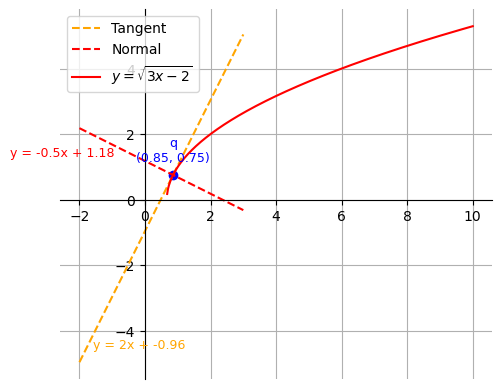
\includegraphics[width=1\textwidth]{plots/plot.png}
    \caption{Tangent and normal to parabola}
    \label{fig:plot}
\end{figure}  
}
\end{document}
